\documentclass[10pt]{beamer}
\usepackage{amsmath}
\usepackage{mathtools}
\usefonttheme{professionalfonts} % using non standard fonts for beamer
\usefonttheme{serif} % default family is serif

%\documentclass[12pt]{beamerthemeSam.sty}
\usepackage{epsf}
%\usepackage{pstricks}
%\usepackage[orientation=portrait,size=A4]{beamerposter}
\geometry{paperwidth=160mm,paperheight=120mm}
%DT favorite definitions
\def\LL{\left\langle}	% left angle bracket
\def\RR{\right\rangle}	% right angle bracket
\def\LP{\left(}		% left parenthesis
\def\RP{\right)}	% right parenthesis
\def\LB{\left\{}	% left curly bracket
\def\RB{\right\}}	% right curly bracket
\def\PAR#1#2{ {{\partial #1}\over{\partial #2}} }
\def\PARTWO#1#2{ {{\partial^2 #1}\over{\partial #2}^2} }
\def\PARTWOMIX#1#2#3{ {{\partial^2 #1}\over{\partial #2 \partial #3}} }

\def\rightpartial{{\overrightarrow\partial}}
\def\leftpartial{{\overleftarrow\partial}}
\def\diffpartial{\buildrel\leftrightarrow\over\partial}

\def\BC{\begin{center}}
\def\EC{\end{center}}
\def\BS{\bigskip}
\def\BI{\begin{itemize}}
\def\EI{\end{itemize}}
\def\BE{\begin{displaymath}}
\def\EE{\end{displaymath}}
\def\BEA{\begin{eqnarray*}}
\def\EEA{\end{eqnarray*}}
\def\BNEA{\begin{eqnarray}}
\def\ENEA{\end{eqnarray}}
\def\EL{\nonumber\\}



\newcommand{\etal}{{\it et al.}}
\newcommand{\gbeta}{6/g^2}
\newcommand{\la}[1]{\label{#1}}
\newcommand{\ie}{{\em i.e.\ }}
\newcommand{\eg}{{\em e.\,g.\ }}
\newcommand{\cf}{cf.\ }
\newcommand{\etc}{etc.\ }
\newcommand{\atantwo}{{\rm atan2}}
\newcommand{\Tr}{{\rm Tr}}
\newcommand{\dt}{\Delta t}
\newcommand{\op}{{\cal O}}
\newcommand{\msbar}{{\overline{\rm MS}}}
\def\chpt{\raise0.4ex\hbox{$\chi$}PT}
\def\schpt{S\raise0.4ex\hbox{$\chi$}PT}
\def\MeV{{\rm Me\!V}}
\def\GeV{{\rm Ge\!V}}

%AB: my color definitions
%\definecolor{mygarnet}{rgb}{0.445,0.184,0.215}
%\definecolor{mygold}{rgb}{0.848,0.848,0.098}
%\definecolor{myg2g}{rgb}{0.647,0.316,0.157}
\definecolor{abtitlecolor}{rgb}{0.0,0.255,0.494}
\definecolor{absecondarycolor}{rgb}{0.0,0.416,0.804}
\definecolor{abprimarycolor}{rgb}{1.0,0.686,0.0}
\definecolor{Red}           {cmyk}{0,1,1,0}
\definecolor{Grey}           {cmyk}{.7,.7,.7,0}
\definecolor{Blue}          {cmyk}{1,1,0,0}
\definecolor{Green}         {cmyk}{1,0,1,0}
\definecolor{Brown}         {cmyk}{0,0.81,1,0.60}
\definecolor{Black}         {cmyk}{0,0,0,1}

\usetheme{Madrid}


%AB: redefinition of beamer colors
%\setbeamercolor{palette tertiary}{fg=white,bg=mygarnet}
%\setbeamercolor{palette secondary}{fg=white,bg=myg2g}
%\setbeamercolor{palette primary}{fg=black,bg=mygold}
\setbeamercolor{title}{fg=abtitlecolor}
\setbeamercolor{frametitle}{fg=abtitlecolor}
\setbeamercolor{palette tertiary}{fg=white,bg=abtitlecolor}
\setbeamercolor{palette secondary}{fg=white,bg=absecondarycolor}
\setbeamercolor{palette primary}{fg=black,bg=abprimarycolor}
\setbeamercolor{structure}{fg=abtitlecolor}

\setbeamerfont{section in toc}{series=\bfseries}

%AB: remove navigation icons
\beamertemplatenavigationsymbolsempty
\title[Newton's Law of Motion]{
  \textbf {Newton's Law of Motion}\\
%\centerline{}
%\centering
%\vspace{-0.0in}
%\includegraphics[width=0.3\textwidth]{propvalues_0093.pdf}
%\vspace{-0.3in}\\
%\label{intrograph}
}

\author[W. Freeman] {Physics 211\\Syracuse University, Physics 211 Spring 2021\\Walter Freeman}

\date{\today}

\begin{document}

\frame{\titlepage}

\frame{\frametitle{\textbf{Announcements}}
\BI
\Large
\item{Homework 3 assigned later today; due next Thursday before class (or maybe Wednesday; stay tuned)}
\item Quiz 1 recap:
\BI
\item Not all the grades are in yet
\item Most folks did very well
\item Anyone who didn't will have another chance later in the term
\EI
\EI

}


\frame{\frametitle{\textbf{Newton's laws}}

\Large

\begin{enumerate}

\item If no net force acts on a thing, its velocity doesn't change: it either keeps moving or keeps not moving, just like it did before

\BS\pause

\item If a net force acts on a thing, it accelerates, with that acceleration equal to the force divided by the thing's mass

\BS\pause

\item If thing A exerts a force on thing B, then thing B exerts a force with the same size in the opposite direction back on thing A.

\end{enumerate}

\Large

\BC
... why is that first one even there? Why are they in that order?
\EC
\pause
\BS
\begin{flushright}...history!\end{flushright}
}
%}
%
%\frame{\frametitle{\textbf{Two revolutions in one!}}
%\Large
%Newton's book {\it Mathematical Principles of Natural Philosophy} was the capstone of two revolutions in one:
%
%\begin{enumerate}
%\item The development of classical mechanics as a way to describe and predict things move
%\item {\color{Red} The emergence of {\it science} as a powerful means to develop models like classical mechanics}
%\end{enumerate}
%
%\large
%
%We're going to spend most of our time learning classical mechanics, but we should spend some time studying 
%science, too!
%
%\BI
%\item What is it?
%\item What does it look like?
%\pause
%\item How does the scientific {\it process} produce revolutions like classical mechanics?
%\item What do other scientific advances look like?
%\pause
%\item What do they {\color{Red} \bf not} look like?
%\pause
%\item How can we ensure that the scientific process is done well and honestly?
%\EI
%}
%
%\frame{\frametitle{\textbf{Aristotelian mechanics}}
%Newton's first law was historically important because it overturned the previous knowledge, from Aristotle:
%
%\BI
%\item Things on Earth that move eventually come to a stop
%\item Things on Earth fall at a constant speed, depending on their weight and the density of the fluid they fall in
%\item Things in the sky don't fall, but move in circles, because they are perfect and heavenly and circles are perfect
%\item How things move is intimately connected to the reasons people (etc.) have for making them move
%\EI
%
%(These first two are actually reasonable in a situation where fluid drag is very large, which is what he studied.)
%}
%
%\frame{\frametitle{\textbf{The new science}}
%
%\Large
%\BC
%What was different about the scientific process?
%\EC
%\BS
%\large
%
%\BI
%\item Primacy of experiment and measurement
%\pause
%\item Seeking truth in {\color{Red} precision} measurements
%\pause
%\item Incorporating things in a unified {\it framework} of laws of nature
%\BI
%\item Natural laws should explain as many things as possible in the same model
%\item Natural laws apply everywhere and for all time
%\EI
%\pause
%\item Awareness of the {\color{Red} limits} of our models, and continually trying to expand them
%\BI
%\item What things do Newton's laws of motion apply to?
%\item How far have we checked them?
%\item Are there any things Newton's laws of motion might {\it not} apply to?
%\EI
%\pause
%\item Science as an {\color{Red} objective} and {\color{Red} non-anthropocentric} explanation:
%\BI
%\item Scientific ideas are bigger than any particular person's perspective; they should be universal
%\item Humans don't have a special role in the laws of nature; if we are special, it's not because we have special rules
%\EI
%\EI
%}
%

\frame{\frametitle{\textbf{Newton's laws}}
    \Large

    \centerline{$\vec F = m\vec a$}
    \large
    \BI
  \item{Forces on an object cause it to accelerate}
  \item{The larger the force, the larger the acceleration}
  \item{The larger the mass, the smaller the acceleration}
  \item{You intuitively know this already}
    \pause
  \item{No forces $\rightarrow$ no acceleration: {\color{Red}not necessarily no motion!}}
    \bigskip
    \bigskip
\item{Forces come in pairs (Newton's third law)}
  \BI
\item{``If A pushes on B, B pushes back on A''}
\item{Very important to be clear about what forces you're talking about}
  \EI
    \EI
   }




   \frame{\frametitle{\textbf{Newtons}}
     \Large{\centerline{We need a new unit for force: the newton}}

     \bigskip
     \bigskip

     \centerline{     $\vec F = m \vec a \rightarrow$ Force has dimensions kg $\rm m/\rm s^2$}
\large
     \bigskip
     \bigskip
\BI
\item{1 N = 1 kg $\rm m/\rm s^2$: about the weight of an apple}

\item{4 N is about a pound}
     \item{9.8 N is the weight of a kilogram}
       \EI
   }

   \frame{\frametitle{\textbf{Force is a vector}}
     \Large
     \centerline{$\vec F = m\vec a$}
     \large
     \BI
   \item{Force is a {\it vector}}
   \item{Multiple forces on an object add like vectors do}
   \item{Really, we should write}

     \Large
     \centerline{$\sum \vec F = m\vec a$}

     \pause
\small

\bigskip
\bigskip
\bigskip
\bigskip
\bigskip

\EI
   }
  \frame{\frametitle{\textbf{Force diagrams}}
  \BI
  \item{Lots of forces, easy to get confused}
  \item{Draw a picture!}
    \centerline{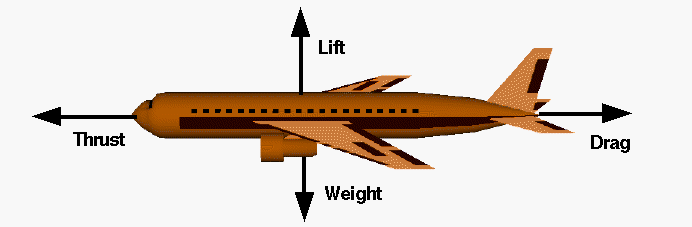
\includegraphics[width=0.6\textwidth]{cruise.png}}
    \pause
  \item{Each object feeling forces gets a separate diagram}
  \item{Label each force and its direction}
  \item{These are also called ``free body diagrams''}
    \EI
  \bigskip
  \bigskip
  \bigskip
  \bigskip
  \pause
  \small


  }


   \frame{\frametitle{\textbf{What is a force?}}
    A force is anything that pushes or pulls something:
    \BI
  \item{Gravity: $F = mg$, so $mg = ma \rightarrow a = g$}
    \BI
  \item{Gravity pulls down on everything (on Earth) with a force $mg$, called its weight}
  \item{If something isn't accelerating downward, some other force must balance its weight}
    \EI
    \EI
  }

  \frame{\frametitle{\textbf{What is a force?}}
    A force is anything that pushes or pulls something:
    \BI
  \item{Gravity: $F = mg$, so $mg = ma \rightarrow a = g$}
  \item{``Normal force'': stops things from moving through each other}
    \BI
  \item{Are there normal forces on me right now?}
 \pause
  \item{However big it needs to be to stop objects from sliding through each other}
  \item{Directed ``normal'' (perpendicular) to the surface}
  \item{Really caused by electric force/Pauli exclusion principle}
    \EI
    \EI
  }


  \frame{\frametitle{\textbf{What is a force?}}
    A force is anything that pushes or pulls something:
    \BI
  \item{Gravity: $F = mg$, so $mg = ma \rightarrow a = g$}
  \item{``Normal force'': stops things from moving through each other}
  \item{Tension: ropes pull on both sides equally}
    \BI
  \item{What are the forces in a contest of tug-of-war?}
    \pause
  \item{What about the forces on the people?}
    \EI
  \item{Friction: a force opposes things sliding against each other}
    \pause
  \item{Electromagnetic forces, nuclear forces, radiation pressure...}
    \pause
  \item{\color{Red}Acceleration is not a force!}
  \item{\color{Red}... it's the {\it result} of forces}
    \EI
  }

\frame{\frametitle{\textbf{One particular force: gravity}}

\Large

Gravity exerts a downward force on all objects (on Earth), with a magnitude of $mg$.

\bigskip

In symbols: $\vec F_g = mg$ downward.

\bigskip
\pause

Why is the acceleration of a falling object $g$ downward?
 
\BI
\item A: Because $g$ is the acceleration of all objects within Earth's gravitational field
\item B: Solve Newton's law: $\vec F = m \vec a \rightarrow mg (-\hat j) = m\vec a \rightarrow \vec a = -g\hat j$
\item C: Because the definition of $g$ is the acceleration that a falling object undergoes
\item D: It's only $g$ if there are no other forces besides gravity acting on it\EI
} 


\frame{
\Large

Suppose an object is moving in a straight line at a constant speed. Which number of forces could {\it not} be 
acting on it?

\BI
\item A: Zero
\item B: One
\item C: Two
\item D: Three
\item E: Four
\EI

\pause

Suppose an object is moving in a circle at a constant speed. Which number of forces could {\it not} be 
acting on it? (Hint: what is the definition of velocity? Of acceleration?)

\BI
\item A: Zero
\item B: One
\item C: Two
\item D: Three
\item E: Four
\EI
}


  \frame{\frametitle{\textbf{Sample questions}}
    \BI
    \Large
  \item{What forces act on a bicycle?}
    \pause
  \item{Which forces are bigger or smaller if it's going at a constant speed?}
    \pause
  \item{Which forces are bigger or smaller if it's slowing down?}
    \pause
  \item{A 100 kg cyclist slows from 10 m/s to a stop over 5 sec. What force is required to do this?}


    \pause

\bigskip
\bigskip
\bigskip
\normalsize
\centerline{(Use $\vec F = m \vec a$ to connect force to acceleration, and then kinematics to connect acceleration to motion)}

    \EI
  }

\frame{\frametitle{\textbf{An important note}}
\large
\BI
\item{Only {\it real physical things} are forces}
\pause
\item{Acceleration is not a force}
\item{``Net force'' is not a force (it's the sum of them)}
\item{Velocity certainly isn't a force}
\pause
\item{If two things don't touch, or interact by gravity, electricity, etc., they don't
exchange forces}
\pause
\item{``A force is something that can send you to the doctor''}
\EI
}

\frame{
\Large
Which of the following is/are {\it not} an example of Newton's third law?

\BI
\item A: a subway car accelerates forward; you are thrown back
\item B: the propeller on an airplane pushes the air backwards; the air pushes the airplane forwards
\item C: an elevator accelerates upward; passengers are pushed downward
\item D: the Earth's gravity pulls downward on me; my gravity pulls upward on the Earth
\item E: a rocket pushes downward on its exhaust; the exhaust pushes upward on the rocket
\EI
}



\frame{\frametitle{\textbf{A sample problem}}
\Large
A stack of two books sits on a table. Each book weighs 10 newtons. Draw a force diagram
for each one, and calculate the size of all the forces.

\bigskip
\bigskip
\bigskip

(Your answer should match what you know about how this works!)
}

  \frame{\frametitle{\textbf{Summary}}
    \Large
    \BI
  \item{Forces: anything that pushes or pulls}
  \item{Forces cause accelerations: $\sum \vec F = m \vec a$}
    \BI
  \item{If $\sum \vec F = 0$, $\vec a = 0$: motion at a constant velocity}
  \EI
  \item{Forces come in pairs: if A pushes on B, B pushes back on A}
  \item{It's the vector sum $\sum \vec F$ that matters}
  \item{Draw force diagrams to keep all of this straight}
    \EI
  }



  \end{document}

